% All I have to read before writing
% https://www.nature.com/srep/author-instructions
% https://www.nature.com/srep/author-instructions/before-you-submit
% https://www.nature.com/srep/author-instructions/submission-guidelines#texlatex-files

\documentclass[fleqn,10pt]{wlscirep}
\usepackage[utf8]{inputenc}
\usepackage[T1]{fontenc}
\title{A fundamental analysis of technological complexity in Japanese corporations}

\author[1,*]{Rintaro Karashima}
\author[1, 2]{Hiroyasu Inoue}
% \author[1,2,+]{Christine Author}
% \author[2,+]{Derek Author}
\affil[1]{University of Hyogo, Graduate School of Information Science, Kobe, 6500047, Japan}
\affil[2]{RIKEN, Center for Computational Science, Kobe, 6500047, Japan}

\affil[*]{rintaro.karashima@gmail.com}

% \affil[+]{these authors contributed equally to this work}

%\keywords{Keyword1, Keyword2, Keyword3}

\begin{abstract}
% Example Abstract. Abstract must not include subheadings or citations. Example Abstract. Abstract must not include subheadings or citations. Example Abstract. Abstract must not include subheadings or citations. Example Abstract. Abstract must not include subheadings or citations. Example Abstract. Abstract must not include subheadings or citations. Example Abstract. Abstract must not include subheadings or citations. Example Abstract. Abstract must not include subheadings or citations. Example Abstract. Abstract must not include subheadings or citations.

\end{abstract}
\begin{document}

\flushbottom
\maketitle
%  <rintaro.karashima@gmail.com> :
%
%  Click the title above to edit the author information and abstract
%
\thispagestyle{empty}

% \noindent Please note: Abbreviations should be introduced at the first mention in the main text – no abbreviations lists. Suggested structure of main text (not enforced) is provided below.

\section*{Introduction}

% The Introduction section, of referenced text\cite{Figueredo:2009dg} expands on the background of the work (some overlap with the Abstract is acceptable). The introduction should not include subheadings.

In the twenty first century, the global landscape of innovation has grown markedly competitive. Nations around the world have designed diverse industrial policies to foster innovation, recognizing it as a vital factor for sustaining economic competitiveness. Despite the abundance of strategies, one persistent challenge remains. It is difficult to identify the core technologies and actors that drive innovation. The difficulty arises from the fact that innovation is an intangible phenomenon emerging from an interconnected ecosystem composed of countries, cities, corporations, and technologies. Understanding this complex environment requires methodologies capable of pinpointing the central elements that contribute to innovation amid intricate interdependencies.
In this context, researchers have recently introduced various indicators to capture the importance of key technological fields in complex environments. Specifically, Hidalgo and Hausmann proposed an approach that measures sophistication by applying network analysis to economic data, and this framework has since been adapted to different areas including patent data. Their Hidalgo Hausmann algorithm has proven instrumental in highlighting technologies and capabilities that hold particular importance [6–10]. Building on this foundation, Balland and Rigby [13] developed the Technological Complexity Index to measure the complexity of technological fields using patent data. This index has informed numerous empirical studies aimed at guiding industrial and innovation policies, especially in the European Union [14–17]. More recently, the method has been extended to Asian contexts and corporate level analyses, supported by increasing availability of detailed patent databases [18–20].

Despite these advancements, comprehensive applications of these methods in the Japanese context remain limited. Japan has experienced prolonged economic stagnation, often described as the Lost Decades, which underscores the urgent need to identify the technologies that will drive renewed innovation and international competitiveness [21]. Although some studies, such as the work on automotive suppliers by Kito[22], have employed related approaches, there is a clear lack of a broad analysis that would illuminate the full landscape of Japanese technologies through the lens of complexity.
This study addresses that gap by applying the Hidalgo Hausmann algorithm to patent data from the Japan Patent Office, focusing on a wide array of technologies held by Japanese corporations. We construct a bipartite network linking corporations and technological fields, and then project it into a monopartite network from which the Technological Complexity Index can be derived. The TCI, represented by the second largest eigenvector of the network adjacency matrix, allows for the simultaneous evaluation of technological spillovers and scarcity. By analyzing trends from 1981 to 2010, this approach provides a stable and finer depiction of the technological landscape that goes beyond conventional quantitative measures such as simple patent counts. In doing so, it captures more nuanced aspects of technological capabilities and their evolution over time.
Ultimately, this research contributes to a deeper understanding of the Japanese innovation ecosystem. By identifying the central fields that drive innovation through the lens of complexity, this study offers valuable insights that can inform more effective policies and strategies. Such insights have the potential to guide Japan toward renewed economic dynamism and a stronger position in the global technological landscape.

The rest of this paper is organized as follows. In the Results section, we present the ubiquity and complexity of technological fields in Japan, followed by a detailed analysis of technological trends. In the Discussion section, we provide a critical analysis of our findings and discuss the implications of our results. 
Finally, in the Methods section, we detail the data processing and methods used in our analysis.

% The paper is organised as follows: in “Data”, we describe the data used in this work and we go through our data cleaning procedure. In “Methods”, we introduce the methodologies used in our work, describing the details of the networks and measures we employed. In “Results”, we discuss the results showing how the network techniques can highlight non-trivial clusters of technologies and metropolitan areas, and how both Fitness and coherent diversifcation are linked to a higher increase in the GDPpc of metropolitan areas. Finally, “Discussion” sums up our contributions and hints at future work needed to address questions arising from this study.

\section*{Results}
% Up to three levels of \textbf{subheading} are permitted. Subheadings should not be numbered.
% In this section, we review the results 

\begin{figure}[ht]
    \centering
    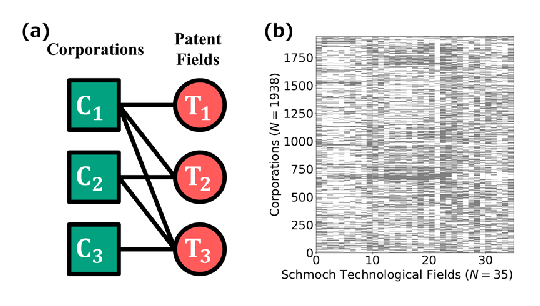
\includegraphics[scale=1]{Figs/Fig1.eps}
    \caption{The bibpartite network of corporations and technological fields. The edges represent that the corporations produce technologies in the fields.}
    \label{fig:bipartite}
\end{figure}

\subsection*{The ubiquity and complexity of technological fields}
Fig. \ref{fig:scatter}a shows the Pearson correlation between the ubiquity \(K_(T,0)\) and the average diversity \(K_(T,1)\) of technological fields, with a correlation coefficient of 0.064. Each point represents a technological field and is color-coded according to the five classifications defined by Schmoch [24]. By plotting the mean values as black lines on both axes, we divided the graph into four quadrants, as shown on the right side of Fig. \ref{}a. In the bottom-left quadrant, we find technologies that are relatively non-ubiquitous and produced by non-diversified corporations, including fields such as Electrical Engineering (e.g. Digital communication, Computer technology, and Semiconductors) and Mechanical Engineering (e.g. Handling, Textile and paper machines, and Thermal pro-cesses and apparatus). Particularly, Electrical Engineering, despite having low degree centrality and average mean neighbor degree, is identified as unsophisticated. This is evident from Fig. 2b, which shows the Pearson correlation between the ubiquity \(K_(T,0)\) and the scaled TCI, with a correlation coefficient of 0.594 like Fig. 2a. This suggests that corporations producing Electrical Engineering technologies focus on producing innovations concentrated within the similar fields rather than engaging with ubiquitous technologies related to other industries, indicating that they have relatively closed portfolios. In contrast, in both panels of Fig. 2, we observe that Chemistry and Pharmaceuticals (e.g. Pharmaceuticals, Organic fine chemistry, and Food Chemistry) are located approximately in the top quadrants. These technologies are non-ubiquitous, highly sophisticated, and produced by relatively diversified corporations. Moreover, this result suggests that corporations producing these technologies are connected not only to non-ubiquitous but also to ubiquitous technologies such as Instruments (e.g. Biotechnology, Analysis of biological materials, and Measurement), which are in the right quadrant of Fig. 2b. Focusing on the IPC classes corresponding to these Schmoch classes, we observed high TCI values in technologies related to the production of sugar (C13) and yeast (A21, C12), drug discovery technologies (A61), and technologies for preserving and managing them (C07, A23). These findings align with the social context of the time such as the dawn of drug discovery or development technologies in the period from the 1980s to the 1990s [28, 29]. Also, food chemistry and biotechnology, which were closely connected to these advancements, played an important role not only in Japan but worldwide during the 1990s to the 2000s, contributing to the development of additives to safely preserve or process food in the food industry [30, 31].

% Example text under a subsection. Bulleted lists may be used where appropriate, e.g.

\begin{figure}[ht]
    \centering
    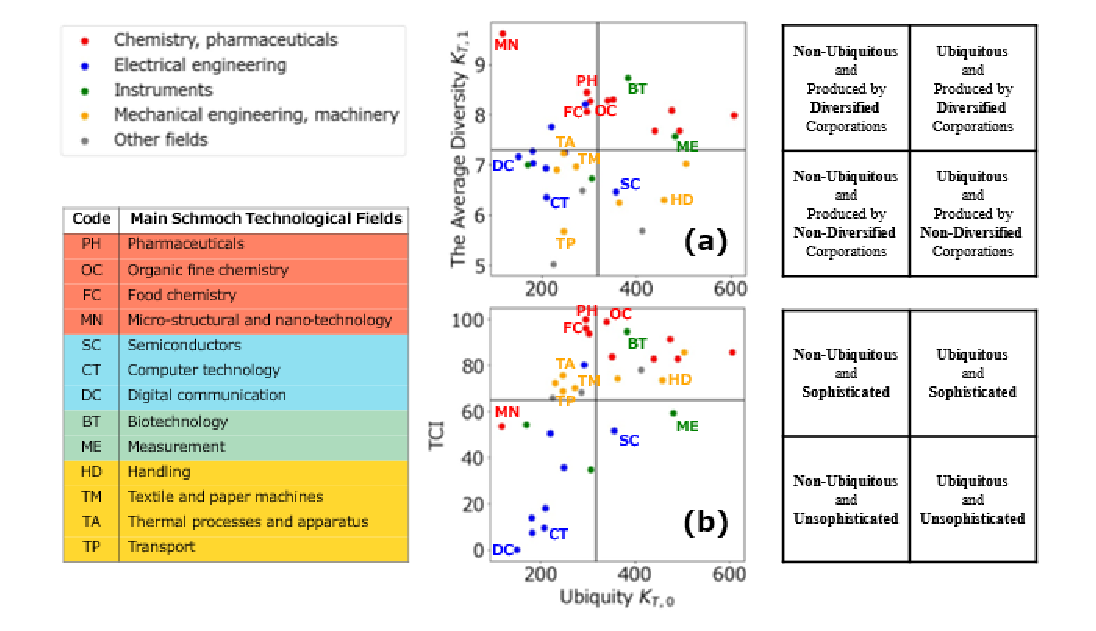
\includegraphics[scale=0.75]{Figs/Fig2.eps}
    \caption{The Pearson correlation between the degree centrality \( k_{t,0} \) of Schmoch technology field node \( t \) and the average nearest neighbor degree \( k_{t,1} \), with a correlation coefficient of 0.064.(a) Similarly, The Pearson correlation between the degree centrality \( k_{t,0} \) of technology field node \( t \) and the Technology Complexity Index (TCI), scaled from 0 to 100, with a correlation coefficient of 0.594. (b) In both figures, the gray dashed lines indicate the mean values. Each data point is color-coded according to the five classifications defined by Schmoch. [Reference]
    All figures were created using Python 3.10 and the matplotlib (3.4.3) package (https://matplotlib.org).}
    \label{fig:scatter}
\end{figure}


\subsection*{More finer technological trends}
\begin{figure}[ht]
    \centering
    \includegraphics[scale=0.75]{Figs/Fig3.eps}
    \caption{The TCI scores of IPC first Class (N=124) and Schmoch (N=35) for both prefectures and corporations.(a) the distribution of the absolute differences between the Technology Complexity Index (TCI) of IPC and the TCI of Schmoch. The scores have been scaled to values ranging from 0 to 100. Each IPC is plotted against the corresponding Schmoch axis, and in cases of many-to-many correspondences, each pair is plotted individually.
    the distribution of the absolute differences between the Technology Complexity Index (TCI) of IPC and the TCI of Schmoch. (b)
    All figures were created using Python 3.10 and the matplotlib (3.4.3) package (https://matplotlib.org).}
    \label{fig:detailtci}
\end{figure}
Fig.\ref{fig:detailtci}a presents the Technology Complexity Index (TCI) for two technology classifications using both the conventional regional approach and the corporate approach introduced in this study. 
To calculate the TCI for the regional approach, a bipartite graph of prefectures and technological fields was constructed using the addresses of corporations.

In the conventional regional approach, the instability of evaluations when using fine classifications, such as IPC classes, has been noted for the regional complexity index, which is paired with the TCI. 
This instability is likely attributable to the symmetry of the bipartite graph, which similarly affects the calculation of the TCI. Specifically, as shown in \ref{fig:detailtci}a, certain technology fields, such as Transport technology, receive markedly different evaluations depending on the classification used, despite belonging to the same technological domain. 
In contrast, the TCI calculated for corporations demonstrates consistent trends when using finer classifications like IPC compared to the Schmoch classification, indicating greater evaluation stability. 
This consistency is further supported by Fig.\ref{fig:detailtci}b, which displays the residuals between the TCI values derived from IPC classes and those from the Schmoch classification, alongside the results of statistical tests for distribution differences.

One possible explanation for this stability in the corporate approach is its ability to quantify ubiquity more precisely than the regional approach. 
In the HH algorithm, ubiquity is defined by the degree of the technological field node. 
However, the range of ubiquity values depends on the number of nodes in the corresponding pair.

\subsection*{Over time variation of finer trends}


\section*{Discussion}

% The Discussion should be succinct and must not contain subheadings.
In this study, we attempted for the first time in Japan to apply the Hidalgo-Hausmann (HH) algorithm to corporations and all patent technology fields, aiming to identify complex and key technological areas. 
The application of the HH algorithm at the corporate level revealed high complexity in the pharmaceuticals and chemistry sectors. This finding may reflect the societal conditions of the time, known as the dawn of the pharmaceutical industry in Japan, indicating a period of significant technological advancement and innovation in these fields.

While some argue that the evaluation results of these technological fields converge due to their classification methods, our corporate approach achieved stable evaluations even when using fine classifications. 
This contrasts with the traditional regional approach, which typically obtains stable evaluations only with coarse classifications. 
The ability of the corporate approach to provide consistent results at a finer granularity suggests its potential to offer more accurate and detailed insights into technological trends within limited spaces, such as specific regions or industries.

However, there remains room to demonstrate the usefulness of this approach in ways that the traditional regional approach has addressed. Capturing changes in technological trends requires not only long-term but also short-term analyses. 
Undertaking such analyses necessitates solving certain data processing challenges. 
Specifically, the calculation of the TCI depends critically on the number of patents by corporation and technology field in each period. 
Shortening the aggregation period may result in the emergence of corporations with a small number of patents which could introduce noise into the TCI calculations and affect the stability of the results.

These limitations may be more effectively addressed through algorithmic improvements rather than ad-hoc measures. 
In the context of complex economics, the HH algorithm which is a linear method dependent on node degrees within the network has been subject to various criticisms and improvements. 
By integrating similar enhancements into our approach, we expect to derive new insights into Japan's industrial technology landscape. 
Future work will focus on comparing the insights obtained through our method with results from applying the corporate approach to patent data from other countries. 
Through this comparative analysis, we aim to contribute to elucidating the characteristics of domestic corporations amid intensifying international competition.

In this study, we conducted the first application of the Technological Complexity Index (TCI) in Japan to identify sophisticated technological fields that are key to fostering innovation. Our findings revealed high sophistication in the pharmaceuticals and chemistry sectors, which may reflect the societal conditions of the time, such as the dawn of the pharmaceutical industry. While some argue that the evaluation results of these technological fields converge due to their classification methods [7], our corporate approach achieved stable evaluations even when using finer classifications or different periods, in contrast to the traditional regional approach. This suggests its potential to offer more accurate and detailed insights into technological trends within limited scopes, such as specific regions or industries. However, there remains room to demonstrate the robustness and usefulness of this approach in ways that the traditional regional method has addressed. Therefore, future work should focus on not only advanced but also empirical analyses, such as comparisons with other countries, verification targeting unexamined specific sectors, and validation of relationships with other innovation indicators.
Also, one of the remaining challenges is the ad-hoc processing of patent data detailed in the previous sections. As we exclude corporations with a small number of patents, it is well argued that fields or corporations with few patents could introduce noise into the accuracy of calculating the TCI and affect the stability of the results [32]. This issue stems from a limitation in the HH algorithm, which evaluates based on the degrees of a bipartite graph, leading to a relaxation of the conditions for link formation. To address this limitation, several mathematical and algorithmic improvements have been proposed [33-35]. In particular, the Fitness-Complexity (FC) algorithm by Tacchella et al. [33], which yields indicators strongly correlated with those obtained by the HH algorithm and regional competitiveness, is widely used in corporate-level analyses. By integrating these enhancements into our approach, we expect to derive new insights into the Japanese industrial technology landscape. Thus, as a cornerstone, this research is expected to be indispensable for elucidating the characteristics of the domestic industry in Japan in an era where AI is on the rise, which is essential for industrial policy.


\section*{Methods}

% Topical subheadings are allowed. Authors must ensure that their Methods section includes adequate experimental and characterization data necessary for others in the field to reproduce their work.
% As Pintar et al.(2022) noted, it is recognised that the use of raw patent counts as measures of innovative output can be problematic because patents' value and importance vary extremely. 
% To remedy this, scholars have analysed the relation of certain additional information that is contained in patent documents with the social and economic value of patents.

%% この期間は日本にとってどんな期間だったか、

%% 特許分類にはIPCを35分類に再編したもの(Schmoch)を用いる
% - These patents encompass a wealth of information, including the identity of the applicant, whether individual or corporate, and their technological domains. 
% For patent classification, this study employs the technological classification proposed by Schmoch (2008), which maps International Patent Classification (IPC) codes onto 35 technological fields.
% We converted the primary IPC classifications onto broader Schmoch categories.\\

% 特許数集計と重み処理
%% 関連文献とは異なり、法人にあたる特許権者の技術分野ごとの特許数を求める
% - Unlike related literature that primarily aggregated data based on the applicant's address and patent classification, 
% this study focuses on corporate patent holders, aggregating data according to patent classification for each corporation.
%% 各法人の技術分野ごとの特許数を求めるうえで、共同出願と複数の技術分野にまたがる特許を考慮する必要がある(関連研究と同様にfractionという言葉を使いたい)
% - we fractionally split individual patents 

% - the granularity of the patent classification used and the method for adjusting the value of each patent. 
% - First, A common approach in related studies was adopted, dividing each patent by the number of classifications it falls under. \\
% - Secondly, unique to this study and not addressed by Pintar et al., 
% was the division of each patent by the number of associated patent holders, 
% an essential element given our focus on corporate aggregations.

% 特許数フィルタ
%% Pintar et al.をはじめとして地域-技術分野グラフから地域の複雑性指標を求めている例では、極端に少ない特許数が指標の算出に影響を与えるとしている。


%% これは、~~ことによるものだと考えられ、二部グラフの対称性より、技術の複雑性指標を求めるうえでも同様のことがいえる。
% - This may cause the inacculately measurement of the TCI. 
%% 実際、より細かい粒度で集計を行っている本研究でも30年間に1つといった極端に少ない特許数を持つ法人がいくつか観測された。
% - Despite the comprehensive 30-year span of collected data, 
% it is noted that some corporations hold significantly fewer patents.

%% そこで私たちは(特許数が少ない法人を除くために)特許数上位3%に絞り込む処理を行った
% To mitigate this, we narrowed to corporations ranked in the top 3\% by patent count, 

% 簡単なデータの記述統計
%% 最終的に対象となったのは1929の法人が35のSchmochにもつ2,800,000件ほどの特許だった。これは全ての法人が持つ特許の約91%に相当する量である。


\subsection*{The bipartite network}
% Hidalgo and Hausmann (2009)は国と製品 → Balland and Rigby (2017)は地域と技術分野 → 本研究は法人と技術分野
% これはIntroductionに入れた方が良い?
Building upon the HH algorithm introduced by Hidalgo and Hausmann (2009)\cite{hidalgo2009eci} for analyzing economic complexity in countries and products, % method of reflectionは使った方がよさそう
Balland and Rigby (2017) have extended this foundational approach to measure the innovation landscape of U.S. regions and technological fields using the Technological Complexity Index (TCI). 
Here, we applied this method to assess Japanese corporations and technology fields. 

% ここの繋がりがちょっと怪しい
% ここからは、RTAと隣接行列の説明
% 「TCIとTCIは二部グラフから求められる」から入った方が良いかも
% RTAはSoete(1987)によって定義されたものという説明が必要
% 閾値はSupporting informationに書く
Currently, there is an active ongoing discussion on the best way to extract information about the (economic) complexity of spatial units from the bipartite network that connects these units to products or knowledge subsets that they produce. In the context of economic complexity of nations, Tacchella et al. (2012) introduced a non-linear iterative algorithm that builds on a similar theoretical basis as Hidalgo and Hausmann (2009) but emphasises that the complexity of products should be more strongly limited by the least fit country that is able to export it. This approach termed Fitness-Complexity Method was shown to produce fitness scores that are strongly associated with economic (Cristelli et al., 2015; Tacchella et al., 2012) and scientific (Cimini et al., 2014) competitiveness of countries. Subsequent studies analysed the mathematical properties (Wu et al., 2016) and conditions for convergence of this algorithm (Pugliese et al., 2016), which revealed some limitations. The convergence of the algorithm to non-zero values for nodes of the network depends highly on the specific network structure. This is expected to be even more problematic when considering the network of technological portfolios than that of trade (Pugliese et al., 2016). Moreover, the strong limiting factor of the least fit exporting country to the complexity of products can lead to an overemphasis on niche products or technological classes. Hence, knowledge subsets in which only very few regions are specialised in could be identified as complex (and consequently their producing regions), even though they are not inherently difficult to produce but only rare (Morrison et al., 2017). For these reasons we focus on the method described in detail above. 
To establish the framework for our analysis, we first determine the Revealed Technological Advantage (RTA) index for each corporation within various technology fields.
The RTA is reflective of a corporation's patent activity in relation to the national standard, and is given by:
This study initiates its analysis by computing the Revealed Technological Advantage (RTA) index for corporations across various patent classifications, reflecting their patent holdings. 
The RTA index, conceptualized as a specialization coefficient by Soete, builds upon Balassa's Revealed Comparative Advantage (RCA) framework. For a given corporation \(c\) within a patent classification \(f\), the RTA index, denoted as \(RTA_{cf}\), is mathematically articulated through the equation:

\[
RTA_{ct} = \frac{X_{ct}}{\sum_{t} X_{ct}} / \frac{\sum_{c} X_{ct}}{\sum_{ct} X_{ct}},
\]

where \(X_{ct}\) signifies the quantity of patents held by corporation \(c\) in category \(t\). The fraction \(\frac{X_{ct}}{\sum_{t} X_{ct}}\) calculates corporation \(c\)'s patent share in classification \(t\), and \(\frac{\sum_{c} X_{ct}}{\sum_{ct} X_{ct}}\) calculates the overall share of patents in classification \(t\) among all corporations. 
Like the RCA index, an RTA index value exceeding a predefined threshold indicates a corporation's technological preeminence in a specific patent classification.

Following the calculation of the \(RTA_{ct}\) matrix, we proceed to construct an adjacency matrix \(M_{ct}\), which serves as the foundation for an unweighted, undirected bipartite graph. This graph is structured around two distinct node types: patent holders and patent classifications, with edges signifying a patent holder's technological dominance within a given classification. In alignment with Soete's methodology, we apply a threshold value of \(R=1\) to discern this dominance:

\[
M_{ct} = 
\begin{cases} 
0 & \text{if } RTA_{ct} < R \\
1 & \text{otherwise}
\end{cases}
\]
\subsection*{Measuring Technological Complexity}

This bifurcation facilitates the definition of two critical metrics: the diversity (\(k_{c,0}\)) of a corporation \(c\) and the ubiquity (\(k_{f,0}\)) of a patent classification \(f\), calculated as:

\[
k_{c,0} = \sum_{t}{M_{ct}},\quad k_{t,0} = \sum_{c}{M_{ct}}.
\]

In the realm of network science, the parameter \(k_{c,0}\) quantifies the degree centrality for corporate nodes, where higher figures indicate a rich complexity and specialization in technology. Conversely, \(k_{t,0}\) assesses the degree centrality for patent classification nodes, with lower figures denoting scarce, highly specialized technologies. 
By exploiting the graph's symmetric properties, we iteratively calculate the average value of adjacent nodes to articulate the distinctive attributes of each corporation and patent classification, where \(N\) denotes the iteration count:

\[
k_{c,N} = \frac{1}{k_{c,0}} \sum_{t} (M_{ct} \cdot k_{t,N-1}),\quad k_{t,N} = \frac{1}{k_{t,0}} \sum_{c} (M_{ct} \cdot k_{c,N-1}).
\]

Next, by substituting equation (5) into equation (4), we obtain equation (6):

\[
k_{c,N} = \frac{1}{k_{c,0}} \sum_{t} \left[ M_{ct} \cdot \frac{1}{k_{t,0}} \sum_{c'} \left( M_{c't} \cdot k_{c',N-2} \right) \right] = \sum_{c'} k_{c',N-2} \cdot \sum_{t} \frac{M_{ct} \cdot M_{c't}}{k_{c,0} \cdot k_{t,0}} = \sum_{c'} M_{c'c} \cdot k_{c',N-2}
\]

Here, \(\widetilde{M}_{tt'}\) which is the adjacency matrix representing the projection of the bipartite graph is defined as:

\[
\widetilde{M_{tt'}} = \sum_{c}{\frac{M_{ct}M_{ct'}}{k_{c,0}k_{t,0}}}
\]

Equation (6) holds when \(k_{c,N} = k_{t',N-2} = 1\), that is, for the eigenvector corresponding to the largest eigenvalue of \(\widetilde{M}_{tt'}\). 
Therefore, this eigenvector, being uniform in component value, is not mathematically informative. 
Conversely, the eigenvector corresponding to the second largest eigenvalue captures the greatest amount of variance. 
Thus, the Technological Complexity Index (TCI) is defined as follows:

\[
TCI = \frac{\vec{T}-<\vec{T}>}{\text{stdev}(\vec{T})}
\]

where \(\vec{T}\) is the eigenvector corresponding to the second largest eigenvalue of \(M_{tt'}\), \(<\vec{T}>\) is the mean of its components, and \(\text{stdev}(\vec{T})\) is the standard deviation of its components. 
Additionally, the TCI of a region is interpreted to be higher when the region has a high diversity and specializes in patent classifications that are less ubiquitous, indicating that the region possesses advanced technologies.

\subsection*{Data}
% 使ったデータの説明
%% Japan Patent Office(JPO)より、1981年度から2010年度に出願された登録済み特許を用いる
Following previous research, we utilize the patent data to map the technological complexity in Japanese corporations.
Specifically, we retrieve the patent registration applied to the Japan Patent Office (JPO) in the period of the fiscal years 1981 to 2010.
For our analysis we use the technological classification proposed by Schmoch (2008) which maps the International Patent Classification (IPC) classes onto 35 fields. 
This classification aims to strike a balance between homogeneity in terms of class sizes and technological homogeneity within each technological field and has been used in related literature with comparable datasets (Balland et al., 2019; Whittle, 2017). 
To construct graphs such as Fig. \ref{fig:bipartite}, it is necessary to calculate how much value each corporation produces in various technological fields. 
Traditional approaches have used the raw number of patents, however, as pointed out by Pintar et al.(2022), the value of patents can vary significantly, making this method problematic. 
Specifically, when a single patent is jointly held by multiple corporations or belongs to multiple technological fields, there is a risk of overestimating the value produced by a corporation. 
To address this issue, we mapped the first IPC class representing the primary field of each patent—to the Schmoch classification system. We then aggregated the data by dividing each patent's value by the number of associated corporations and the number of technological fields it encompasses.

At this stage, the dataset comprised 2.5 million patents held by 80,000 corporations. Despite the extensive 30-year aggregation period, we observed corporations with a minimal number of patents, such as a single patent in one field. 
Including these corporations could overly simplify the conditions for link formation in the graph construction required by the HH algorithm, which is why previous studies have excluded them. 
Based on the distribution of patent counts per corporation, we filtered the dataset to include patents held by the top 3\% of corporations.
The final dataset consisted of 2.48 million patents held by 1,938 corporations, representing approximately 93\% of the patents before filtering.



\bibliography{ref}

% \noindent LaTeX formats citations and references automatically using the bibliography records in your .bib file, which you can edit via the project menu. Use the cite command for an inline citation, e.g.  \cite{Hao:gidmaps:2014}.

% For data citations of datasets uploaded to e.g. \emph{figshare}, please use the \verb|howpublished| option in the bib entry to specify the platform and the link, as in the \verb|Hao:gidmaps:2014| example in the sample bibliography file.

% \section*{Acknowledgements (not compulsory)}
% Acknowledgements should be brief, and should not include thanks to anonymous referees and editors, or effusive comments. Grant or contribution numbers may be acknowledged.

\section*{Author contributions statement}
R.K. collected and analysed the data. All authors designed the research, wrote and reviewed the manuscript.
% Must include all authors, identified by initials, for example:
% A.A. conceived the experiment(s),  A.A. and B.A. conducted the experiment(s), C.A. and D.A. analysed the results.  All authors reviewed the manuscript. 

\section*{Additional information}

To include, in this order: \textbf{Accession codes} (where applicable); \textbf{Competing interests} (mandatory statement). 

The corresponding author is responsible for submitting a \href{http://www.nature.com/srep/policies/index.html#competing}{competing interests statement} on behalf of all authors of the paper. This statement must be included in the submitted article file.

% \begin{figure}[ht]
% \centering
% 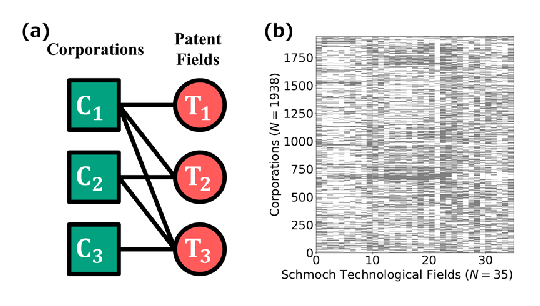
\includegraphics[width=\linewidth]{Figs/Fig1.eps}
% \caption{Legend (350 words max). Example legend text.}
% \label{fig:stream}
% \end{figure}

% \begin{table}[ht]
% \centering
% \begin{tabular}{|l|l|l|}
% \hline
% Condition & n & p \\
% \hline
% A & 5 & 0.1 \\
% \hline
% B & 10 & 0.01 \\
% \hline
% \end{tabular}
% \caption{\label{tab:example}Legend (350 words max). Example legend text.}
% \end{table}

% Figures and tables can be referenced in LaTeX using the ref command, e.g. Figure \ref{fig:stream} and Table \ref{tab:example}.



% Example text under a subsection. Bulleted lists may be used where appropriate, e.g.


% 遍在性が低い特許分類の特徴
% - 最も複雑な技術は次数がある程度低いが、必ずしも最低ではない。
% - 逆に、当時広く生産されていなかったコンピューティングと電子技術のような次数が低いがTCIが低いような技術も見られた。


% 複雑性が高い特許分類の特徴
% - 高いTCI (>80) を持つ技術(Pharmaceuticals, Chemistry系)は、技術の量を表す特許数での評価では低~中程度の評価がなされている。また
% - 中程度のTCI (60 < TCI < 80) を持つ技術()。

% - 特許数とKCIの関連(Appendix)
%    - 特許とKCIのスピアマン順位相関: 。
%    - 特許数が高いがTCIが低い技術()。
%    - TCIが特許数よりも高い技術()。

% table1: 全schmochの特許数、次数、TCI
% \begin{table}[ht]
%     \centering
%     % \caption{Technological complexity of 35 fields}
%     % \label{tab:tciofclass}
%     \caption{\label{tab:tciofclass}Technological complexity of 35 fields}
%     \begin{tabular}{lllll}
%         \toprule
%         % Technological Fields & Registration counts & Registration counts rank & Degree centrality & TCI \\
%         Technological Fields & Registration counts & Registration counts rank & Ubiquity & TCI \\
%         \midrule
%         Pharmaceuticals & 13832.9 & 32 & 295 & 100.00 \\
%         Organic fine chemistry & 49762.8 & 24 & 339 & 98.98 \\
%         Food chemistry & 19104.5 & 30 & 295 & 96.06 \\
%         Biotechnology & 18842.5 & 31 & 382 & 94.65 \\
%         Macromolecular chemistry, polymers & 73747.9 & 18 & 302 & 93.81 \\
%         Basic materials chemistry & 49795.8 & 23 & 474 & 91.40 \\
%         Analysis of biological materials & 6928.9 & 34 & 372 & 89.64 \\
%         Other special machines & 97979.1 & 11 & 504 & 85.77 \\
%         Chemical engineering & 48801.5 & 25 & 606 & 85.56 \\
%         Materials, metallurgy & 96984.9 & 12 & 351 & 83.89 \\
%         Surface technology, coating & 70207.9 & 19 & 490 & 82.93 \\
%         Environmental technology & 42906.5 & 27 & 439 & 82.82 \\
%         Medical technology & 60318.6 & 21 & 292 & 80.15 \\
%         Civil engineering & 112115.7 & 8 & 412 & 78.15 \\
%         Thermal processes and apparatus & 67397.1 & 20 & 247 & 75.65 \\
%         Machine tools & 91314.7 & 16 & 417 & 74.51 \\
%         Mechanical elements & 74104.7 & 17 & 363 & 74.13 \\
%         Handling & 94923.8 & 15 & 458 & 73.63 \\
%         Engines, pumps, turbines & 95954.6 & 14 & 231 & 72.43 \\
%         Textile and paper machines & 99098.6 & 10 & 272 & 70.26 \\
%         Transport & 136292.5 & 7 & 247 & 68.73 \\
%         Other consumer goods & 46413.0 & 26 & 286 & 68.22 \\
%         Furniture, games & 96747.0 & 13 & 225 & 65.96 \\
%         Measurement & 157480.2 & 4 & 481 & 59.25 \\
%         Optics & 210773.1 & 2 & 170 & 54.33 \\
%         Micro-structural and nano-technology & 758.3 & 35 & 117 & 53.54 \\
%         Electrical machinery, apparatus, energy & 218723.6 & 1 & 356 & 51.73 \\
%         Semiconductors & 139489.6 & 6 & 220 & 50.34 \\
%         IT methods for management & 8681.0 & 33 & 249 & 35.62 \\
%         Control & 53045.5 & 22 & 306 & 34.69 \\
%         Audio-visual technology & 185920.5 & 3 & 210 & 17.97 \\
%         Basic communication processes & 35135.6 & 29 & 181 & 13.76 \\
%         Computer technology & 150378.0 & 5 & 208 & 9.58 \\
%         Telecommunications & 100147.3 & 9 & 182 & 7.41 \\
%         Digital communication & 36549.1 & 28 & 150 & 0.00 \\
%         \bottomrule
%     \end{tabular}
% \end{table}

\end{document}